\section{Theorie}
\label{sec:theorie}

Im folgenden Abschnitt sollen die theoretischen Grundlagen der Wechselwirkung von hochenergetischer Strahlung mit Materie
sowie die Funktionsweise des Germaniumdetektors erläutert werden.


\subsection{Wechselwirkung von Strahlung mit Materie}
\label{sec:wechselwirkungen}

Wenn hochenergetische $\gamma$-Strahlung auf Materie trifft,
treten,
abhängig von der Energie der Strahlung,
unterschiedliche Effekte auf.
Die Zahl der Photonen $N(d)$ in Abhängigkeit der Eindringtiefe $d$ ist durch den Zusammenhang
\begin{equation}
    N(d) = N_0 \cdot \symup{e}^{-\mu \cdot d}
\end{equation}
gegeben.
Der Faktor $\mu = n \cdot \sigma$ beschreibt den Extinktionskoeffizienten,
mit dem Wirkungsquerschnitt $\sigma$ des jeweiligen Prozesses und $n$ der Anzahl Elektronen pro Probenvolumen.
Aufgrund der unterschiedlichen Dominanz der Effekte abhängig von der Energie der $\gamma$-Strahlung ergibt sich auch eine Energieabhängigkeit des Extinktionskoeffizienten.
Diese ist in \autoref{fig:extinktionskoeffizient} dargestellt.
\begin{figure}
    \centering
    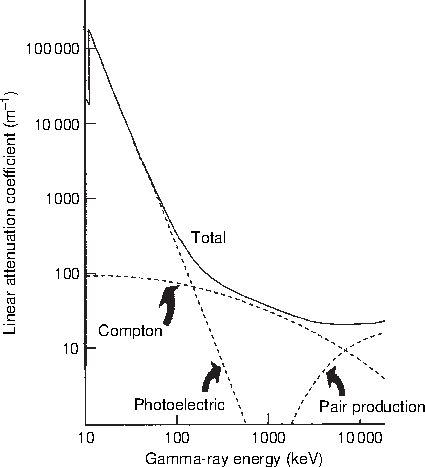
\includegraphics[width=0.5\textwidth]{content/img/Gilmore_Abb_2.3.pdf}
    \caption{Verlauf des Extinktionskoeffizienten in Abhängigkeit der Energie der $\gamma$-Strahlung \cite{gilmore}.}
    \label{fig:extinktionskoeffizient}
\end{figure}

Für Photonenergien von $E_{\gamma} \approx \SI{100}{\kilo\eV}$ dominiert der \textbf{Photoeffekt}.
Dabei wird das Photon von einem Atom vollständig absorbiert und kann ein Elektron herauslösen,
wenn die Energie des Photons größer als die Bindungsenergie $E_\text{Bind}$ des Elektrons ist.
Das herausgelöste Elektron behält die Energie $E_\text{e} = E_{\gamma} - E_\text{Bind}$ zurück.
Im Atom entsteht eine Lücke in der entsprechenden Schale,
welche durch ein Elektron von einer anderen Schale gefüllt werden kann.
Dabei entsteht ein weiteres Photon mit der entsprechenden Energiedifferenz.
Für den Wirkungsquerschnitt des Photoeffekts gilt
\begin{equation*}
    \sigma_\text{Photo} \propto \frac{Z^n}{E^{\sfrac{7}{2}}_{\gamma}}
\end{equation*}
mit der Ordnungszahl $Z$ des Atoms und $4 \leq n \leq \num{5}$.

Für höhere Photonenergien dominiert der \textbf{Compton-Effekt}.
Dabei stößt das Elektron mit einem Elektron und überträgt einen Teil der Energie auf das Elektron,
welcher abhängig vom Streuwinkel $\theta$ ist.
Die Energie des Photons nach dem Stoß kann mit
\begin{equation*}
    E^{'}_{\gamma} = \frac{E_{\gamma}}{1 + \epsilon(1 - \cos{\theta})}
\end{equation*}
berechnet werden,
wobei $\epsilon = \sfrac{E_{\gamma}}{m_\text{e} c^2}$ ist,
mit der Ruhemasse $m_\text{e}$ des Elektrons.
Da $\theta$ kontinuierliche Werte annehmen kann,
ist auch der Energieübertrag zwischen Photon und Elektron kontinuierlich.
Bei einem Streuwinkel von $\theta = \pi$ findet ein maximaler Energieübertrag statt;
das Elektron hat nach dem Stoß eine Energie von
\begin{equation*}
    E_\text{e} = \frac{2 \epsilon}{1 + 2 \epsilon} \ .
\end{equation*}
Im Spektrum des $\gamma$-Strahlers findet sich an dieser Stelle die Compton-Kante,
während die übrigen Energien in Form eines Compton-Kontinuums sichtbar sind.
Der Wirkungsquerschnitt des Compton-Effekts ergibt sich über eine Winkelintegration der \emph{Klein-Nishina-Gleichung} \cite{knoll}.
Es gilt
\begin{equation}
    \sigma_\text{Compton} =
    2 \pi r^2_\text{e} \left(\frac{1+\epsilon}{\epsilon} \left(\frac{1+2\epsilon}{2\epsilon} - \frac{1}{\epsilon}\ln(1+2\epsilon)\right)\right)
    + \frac{1}{2\epsilon} \ln(1+2\epsilon) - \frac{1+3\epsilon}{(1+2\epsilon)^2} \ .
\end{equation}

Ein weiterer möglicher Prozess ist durch \textbf{Paarbildung} gegeben.
Diese tritt erst für Photonenergien $E_{\gamma} \geq 2 m_\text{e} c^2 \approx \SI{1.022}{\mega\eV}$ auf.
Im Coulombfeld eines Atomkerns wandelt sich das Photon in ein Elektron-Positron-Paar um,
wobei Elektron und Positron die übrige Energie des Photons als kinetische Energie zurückbehalten.
Der Wirkungsquerschnitt für diesen Prozess verhält sich wie
\begin{equation*}
    \sigma_\text{Paar} \propto Z^2 f(Z, E_{\gamma}) \ .
\end{equation*}

Das charakteristische Spektrum eines $\gamma$-Strahlers ist beispielhaft in \autoref{fig:spektrum} dargestellt,
wobei je nach Auflösungsvermögen des Detektors der Rückstreupeak,
die Compton-Kante,
sowie das Compton-Kontinuum und der Photopeak sichtbar sind.
Der Rückstreupeak entsteht dabei durch Compton-Effekt in der Detektorumgebung,
dessen Signal trotzdem detektiert wird.
%TODO: Geeignete Abbildung finden (Vllt die von V14 zu der Cs-Quelle?)
\begin{figure}
    \centering
    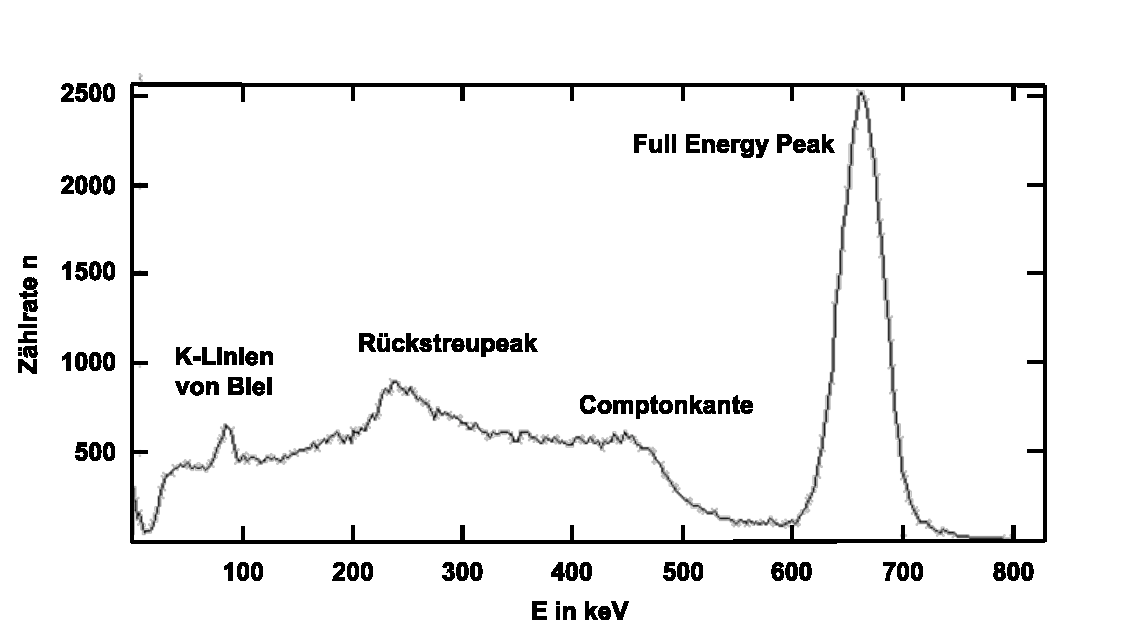
\includegraphics[width=\textwidth]{content/img/cs137-spektrum_Leifi.pdf}
    \caption{
        Charakteristisches Spektrum eines $\ce{^137Cs}$-Strahlers \cite{caesium}.
        Erkennbar sind der Rückstreupeak,
        die Compton-Kante und der Photopeak.
    }
    \label{fig:spektrum}
\end{figure}


\subsection{Funktionsweise des Germaniumdetektors}
\label{sec:funktionsweise}

Germanium ist ein indirekter Halbleiter,
welcher in der $\gamma$-Spektroskopie verwendet wird,
da er eine besonders gute Energieauflösung besitzt \cite{kolanoskiwermes}.

Der Germaniumdetektor besteht aus einem Germanium-Kristall,
dessen eine Seite mithilfe von n-dotiert ist,
während die andere Seite des Detektors p-dotiert ist.
Aufgrund der unterschiedlichen Dotierung entsteht eine Verarmungszone,
da die überschüssigen Löcher und Elektronen im Material rekombinieren.
Trifft nun $\gamma$-Strahlung auf den Detektor,
finden abhängig von der Energie der Strahlung die in \autoref{sec:wechselwirkungen} beschriebenen Prozesse statt.
Bei diesen entstehen freie Elektronen,
welche mit den gebundenen Elektronen des Kristalls stoßen.
Wenn der Energieübertrag beim Stoß groß genug ist,
können die gebundenen Elektronen aus dem Valenzband in das Leitungsband gehoben werden.
Im Valenzband entstehen so weitere Löcher,
sodass sich die Löcher und Elektronen im Valenz- und Leitungsband umverteilen.
Dies kann als Strom gemessen werden.

Damit möglichst viele $\gamma$-Quanten nachgewiesen werden können,
sollte die Verarmungszone möglichst breit sein.
Dies ist über Anlegen einer externen Spannung
oder durch eine asymmetrische Dotierung möglich.
Aufgrund von weiteren Elektronübergängen in einem Halbleiter bei einer Temperatur größer Null entstehen zusätzliche Ströme,
welche die Messung der von $\gamma$-Strahlung erzeugten Ströme stören.
Um diese ungewollten Ströme zu verringern,
wird der Detektor gekühlt.
Die Detektoreffizienz $Q$ wird durch
\begin{equation}
    Q = \frac{4 \symup{\pi} N}{\Omega A W t_\text{m}}
    \label{eqn:effizienz}
\end{equation}
beschrieben,
mit dem Raumwinkel $\Omega$,
der Zählrate $N$,
der Aktivität $A$ und der Messdauer $t_\text{m}$.
